\documentclass[11pt]{report}

\usepackage{graphicx}

\begin{document}

\title{CS663 Assignment-5 Question-2 Report}
\author{KOTWAL ALANKAR SHASHIKANT | 12D070010}
\maketitle

\section*{Image 1}
The filtered result is the following: (original image on the left, filtered version on the right)
\newline \newline
\centerline{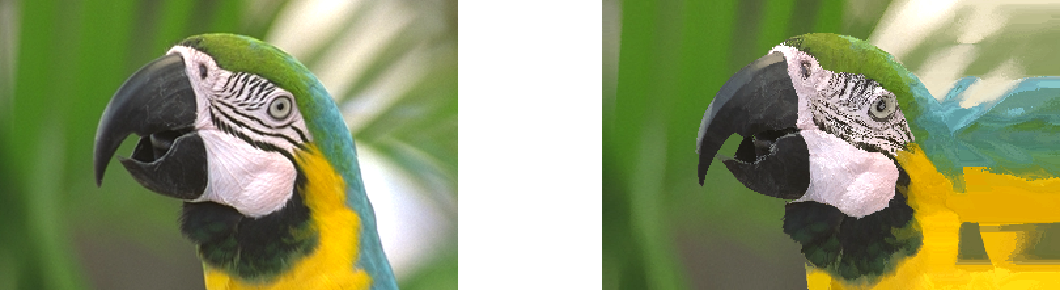
\includegraphics[scale=0.5]{parrot_filtered.png}}
\newline \newline
After doing segmentation, the output is as follows:
\newline \newline
\centerline{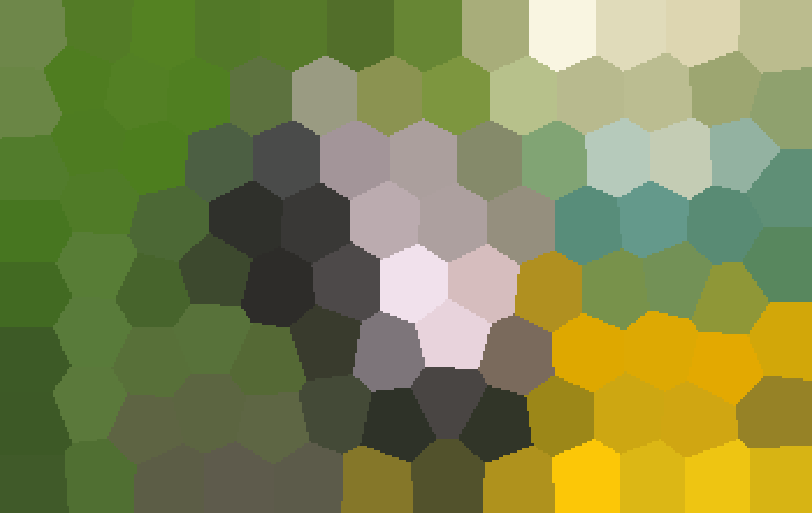
\includegraphics[scale=0.5]{parrot_segmented.png}}

\newpage

\section*{Image 2}
The filtered result is the following: (original image on the left, filtered version on the right)
\newline \newline
\centerline{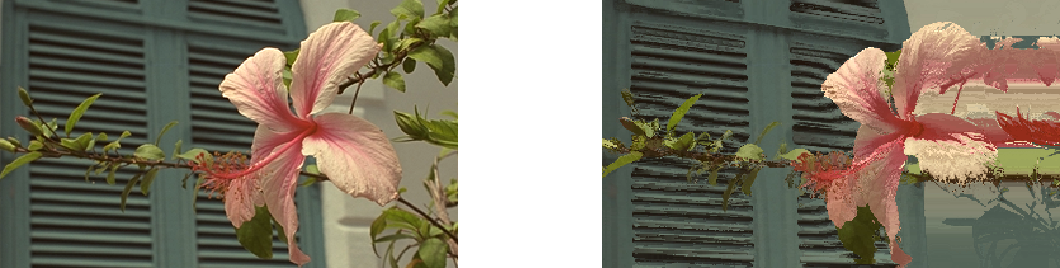
\includegraphics[scale=0.5]{flower_filtered.png}}
\newline \newline
After doing segmentation, the output is as follows:
\newline \newline
\centerline{
\includegraphics[scale=0.5]{flower_segmented.png}}
\newline \newline \newline \newline
Note that the code takes a long time ($\sim$ 30 minutes) to run.

\end{document}